\documentclass{beamer}

\usepackage[utf8x]{inputenc}
\usepackage{default}

\usepackage[slovene]{babel}
\date{21. marec 2012}

\title{Hidrodinamske nestabilnost v tankih plasteh}
\author{Miha \v Can\v cula}

\renewcommand{\vec}{\mathbf}


\begin{document}

\frame{\titlepage}

\begin{frame}{Vsebina}
 \begin{itemize}
  \item Stabilnost
  \item Ena"cbe toka teko"cin
  \item Lubrikacijski pribli"zek -- ena"cba tankega filma
  \item Primeri
  \begin{itemize}
    \item{Plast teko"cine na klancu}
    \item{Razpad milnega mehur"cka}
    \item{Nastanek kra"skih "zlebi"cev}
  \end{itemize}
 \end{itemize}
\end{frame}


\begin{frame}{Stabilnost}
\begin{block}{Osnovna re"sitev}
 \begin{itemize}
  \item Ohranja simetrijo ena"cbe
 \end{itemize}
\end{block}

\begin{block}{Motnja}
 \begin{itemize}
 \item Kr"si simetrijo
 \item Majhna v primerjavi z osnovno re"sitvijo
 \end{itemize}
 \end{block}
 
 \begin{block}{Stabilnost}
 \begin{itemize}
  \item Majhna motnja po dolgem "casu ostane majhna
 \end{itemize}
 \end{block}

\end{frame}

\begin{frame}{Ena"cbe}

\begin{block}{Navier-Stokes}
\[ \frac{\partial \vec u}{\partial t} + (\vec u \cdot \nabla) \vec u = -\frac{1}{\rho}\nabla p + \mu \Delta \vec u \] 
\end{block}
\begin{block}{Brezdimenzijska}
\[ \frac{\partial \vec U}{\partial t} + (\vec U \cdot \nabla) \vec U = -\nabla P + R^{-1}\Delta \vec U \] 
\end{block}
\begin{block}{Nestisljivost}
\[ \nabla \vec u = 0 \]
\end{block}

\end{frame}

\begin{frame}{Lubrikacijski pribli"zek}
 \begin{block}{Predpostavke}
  \begin{itemize}
   \item Zna"cilna dimenzija v smeri $z$ mnogo manj"sa
   \item Hitrost v tej smeri majhna, $u_z \ll u_x, u_y$. 
  \end{itemize}
  \end{block}
  
  \begin{block}{U"cinek}
  \begin{itemize}
   \item Povpre"cenje v $z$ smeri $\Rightarrow$ izgubimo profil v $z$ smeri
   \item Menjava spremenljivke $\vec u(x,y,z,t) \to h(x,y,t)$
   \item 4 skalarne koli"cine ($\vec u, p$) $\to$ 1 skalarna koli"cina. 
   \end{itemize}
 \end{block}
\end{frame}

\begin{frame}{Lineariziran problem}
\begin{itemize}
 \item $ h(x,y,t) = h_0(x,t) + \varepsilon h_1(x,y,t) $, \; $\varepsilon \ll 1$, \; $h_1 \sim h_0$
 \item Re"simo $h_0$ $\rightarrow$ ena"cba za $h_1$
 \item Razvoj po $\varepsilon$, obdr"zimo le do linearnega "clena
\end{itemize}

\end{frame}

\begin{frame}{Plast teko"cine na klancu}
 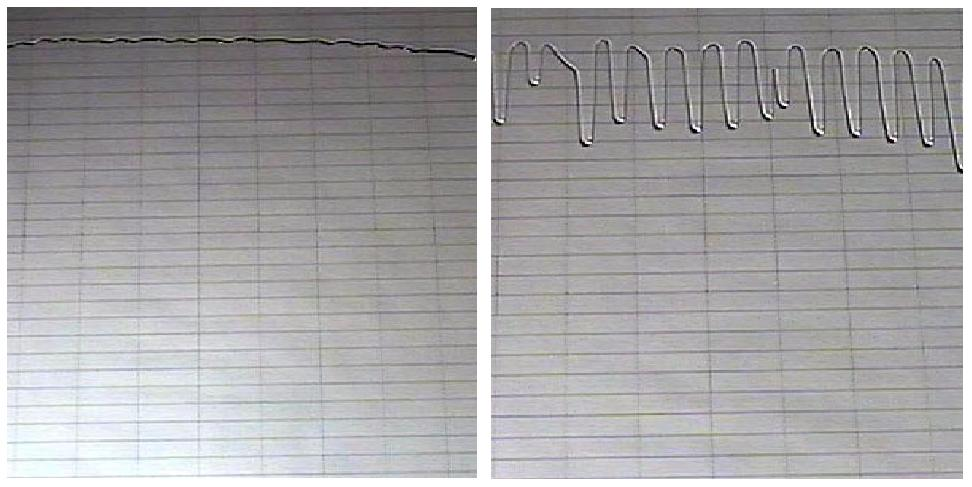
\includegraphics[width=\textwidth]{./Slike/film-slika}
\end{frame}

\begin{frame}{Stabilnost}
 
\end{frame}

\begin{frame}{Razpad milnega mehur"cka}
\begin{center}
 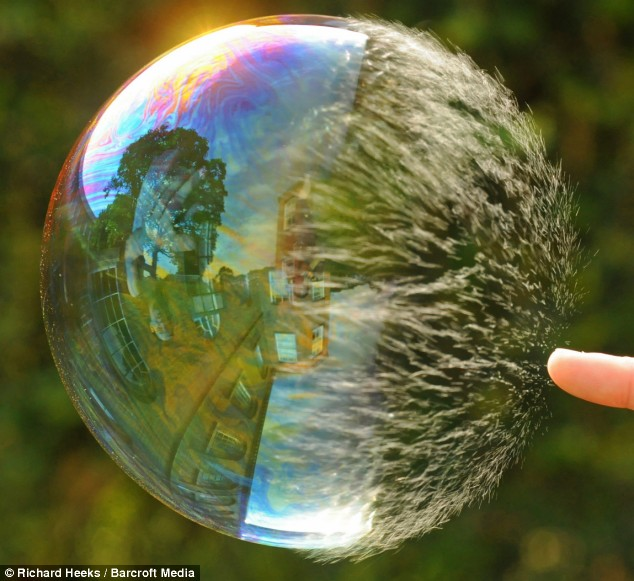
\includegraphics[width=.8\textwidth]{./Slike/bubble-3}
\end{center}
\end{frame}

\begin{frame}{Tanka opna}
 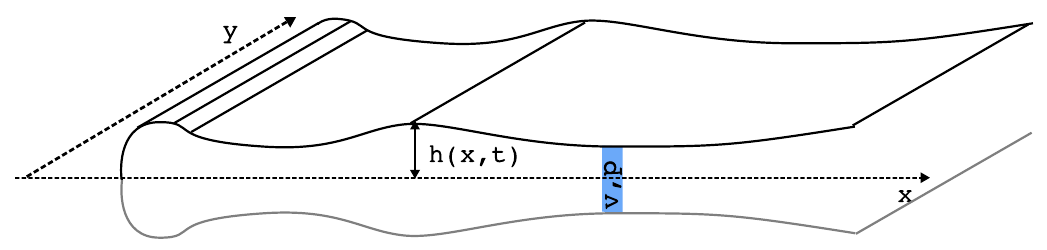
\includegraphics[width=.8\textwidth]{./Slike/mehurcek-skica}
 \begin{itemize}
  \item Neuravnove"sena povr"sinska napetost
  \item Lubrikacijski pribli"zek
  \item Dve simetriji: $y$ in $x-ct$
  \item Nestabilnost = razpad na kapljice
  \item Klju"cen parameter: viskoznost
 \end{itemize}

\end{frame}

\begin{frame}{Neviskozna opna}
 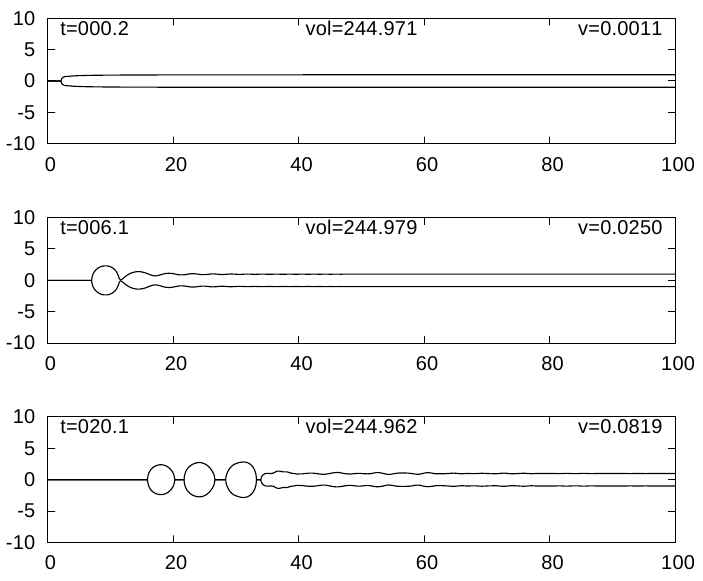
\includegraphics[height=.5\textheight]{./Slike/mehurcek-rezultat-1}
 \begin{itemize}
  \item Razpad simetrije v smeri $x$ $\Rightarrow$ razpad opne v valje
  \item Valji naprej razpadejo v kapljice
 \end{itemize}

\end{frame}

\begin{frame}{Viskozna opna}
 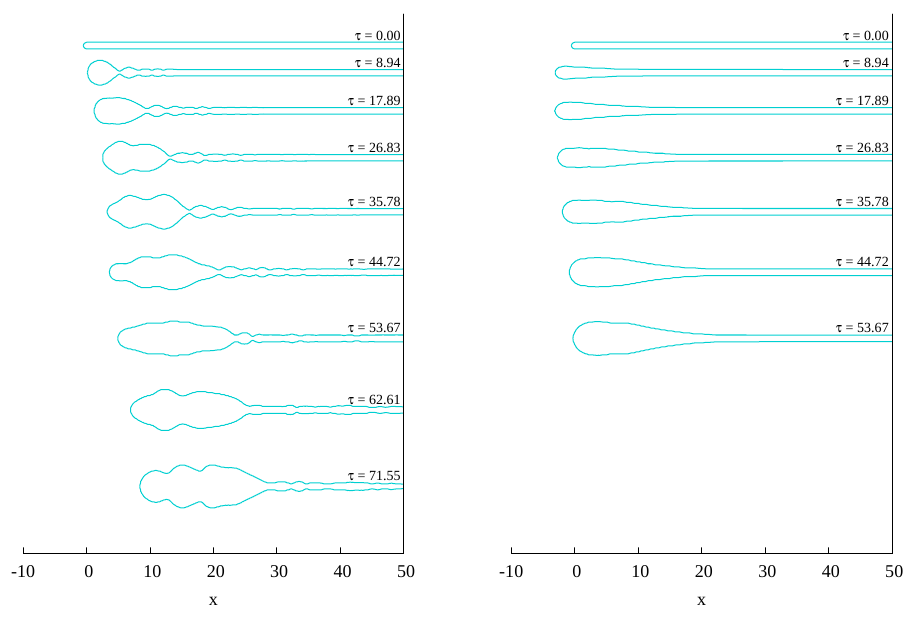
\includegraphics[width=.7\textwidth]{./Slike/scat-rezultat-1}
 \begin{itemize}
  \item Po"casnej"se umikanje roba
  \item Opna ne razpade
 \end{itemize}
\end{frame}
 
\begin{frame}{Kra"ski "zlebi"ci}
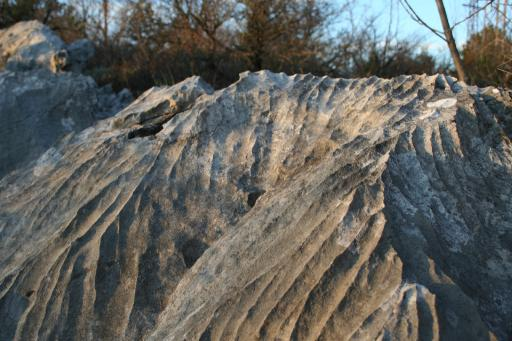
\includegraphics[width=\textwidth]{./Slike/Zlebici}

\end{frame}

\begin{frame}{Kra"ski "zlebi"ci}
  \begin{block}{Nastanek}
  \begin{itemize}
    \item Na kra"skih pobo"cjih
    \end{itemize}
  \end{block}
  
  \begin{block}{Nestabilnost}
  \begin{itemize}
    \item Majhna motnja v obliki povr"sja se poglablja
    \end{itemize}
  \end{block}

\end{frame}


\end{document}
